\documentclass[11pt]{article}
\usepackage[T1]{fontenc}
\usepackage{lmodern}
\usepackage[margin=1in]{geometry}
\usepackage{amsmath,amssymb,amsthm,mathtools}
\usepackage{microtype}
\usepackage{booktabs}
\usepackage{enumitem}
\usepackage[dvipsnames]{xcolor}
\usepackage{tikz}
\usetikzlibrary{positioning,arrows.meta,fit,calc,shapes.geometric}
\usepackage[most]{tcolorbox}
\usepackage{caption}
\usepackage[colorlinks=true,linkcolor=MidnightBlue,urlcolor=MidnightBlue,citecolor=MidnightBlue]{hyperref}

\theoremstyle{definition}
\newtheorem{definition}{Definition}[section]
\newtheorem{example}[definition]{Example}
\newtheorem{remark}[definition]{Remark}
\theoremstyle{plain}
\newtheorem{proposition}[definition]{Proposition}
\newtheorem{lemma}[definition]{Lemma}
\newtheorem{theorem}[definition]{Theorem}
\theoremstyle{definition}
\newtheorem{exercise}{Exercise}

\newcommand{\C}{\mathbb{C}}
\newcommand{\R}{\mathbb{R}}
\newcommand{\U}{\mathrm{U}}
\newcommand{\SU}{\mathrm{SU}}
\newcommand{\inner}[2]{\langle #1,#2\rangle}
\newcommand{\abs}[1]{\lvert #1\rvert}
\newcommand{\norm}[1]{\lVert #1\rVert}
\newcommand{\Frob}{\mathrm{F}}
\newcommand{\op}{\mathrm{op}}
\newcommand{\dd}{\mathrm{d}}
\DeclareMathOperator{\tr}{tr}
\DeclareMathOperator{\rank}{rank}
\DeclareMathOperator{\diag}{diag}

% boxes
\newtcolorbox{ideabox}[1][]{colback=MidnightBlue!4,colframe=MidnightBlue!55!black,
  fonttitle=\bfseries,title=The idea in one paragraph,#1}
\newtcolorbox{paperbox}[1][]{colback=Gray!6,colframe=Gray!55!black,
  fonttitle=\bfseries,title=Where this is in the paper,#1}
\newtcolorbox{warnbox}[1][]{colback=Orange!4,colframe=Orange!70!black,
  fonttitle=\bfseries,title=Watch the direction of the implication,#1}
\newenvironment{claim}{\begin{quote}\itshape}{\end{quote}}

\title{\bfseries Why $\C^6$ has only three unbiased bases\\[4pt]
\large The high-level shape of a computer-assisted proof,\\ for a reader who has taken one course in linear algebra}
\author{Reading notes on\\[2pt]
OpenAI, \emph{The maximum number of mutually unbiased bases in dimension six}\\[2pt]
{\small preprint dated 24 September 2026; these notes cover its first fifteen pages}}
\date{}

\begin{document}
\maketitle

\begin{abstract}
\noindent
A family of orthonormal bases of $\C^6$ is called \emph{mutually unbiased} when any two of them
are as unrelated as two bases can be. Three such bases are easy to write down; a 1991 conjecture
of Zauner says that a fourth cannot exist. The preprint outlines a proof of that conjecture in
which the continuous problem --- one $6\times6$ matrix with $36$ free phases --- is turned into
finitely many finite computations, each of which either rules its region out or hands the region
to a smaller, better region. These notes describe that reduction and nothing else: the sequence
of ideas, the one logical invariant that holds the proof together, and the reason each technical
estimate is there. They are meant to be readable with only linear algebra in $\C^d$, and they
deliberately omit the arithmetic bookkeeping that occupies most of the paper.
\end{abstract}

\tableofcontents

\bigskip

\section{Two bases that tell you nothing about each other}

\begin{definition}[Unbiased pair of bases]\label{def:mub}
Let $\mathcal B=(b_1,\dots,b_d)$ and $\mathcal C=(c_1,\dots,c_d)$ be orthonormal bases of $\C^d$.
They are \emph{mutually unbiased} (or simply \emph{unbiased}) if
\begin{equation}\label{eq:mub}
\abs{\inner{b_i}{c_j}}^2=\frac1d
\qquad\text{for all } i,j\in\{1,\dots,d\}.
\end{equation}
A family $\mathcal B_0,\dots,\mathcal B_{m-1}$ of orthonormal bases is mutually unbiased if every
pair of them is. Write $N(d)$ for the largest $m$ for which such a family exists.
\end{definition}

Throughout, $\inner{u}{v}=\sum_j\overline{u_j}v_j=u^*v$, conjugate-linear in the first slot and linear
in the second, as in the preprint. The modulus, not the phase, appears in \eqref{eq:mub}, and that is
the point. Write $P_{ij}=\abs{\inner{b_i}{c_j}}^2$.
Because $c_j$ is a unit vector and $\mathcal B$ is an orthonormal basis, Pythagoras in $\mathcal B$ gives
$\sum_i P_{ij}=1$; because $b_i$ is a unit vector and $\mathcal C$ is an orthonormal basis,
$\sum_j P_{ij}=1$. So $P$ is a \emph{doubly stochastic} $d\times d$ matrix, and
\eqref{eq:mub} says that $P$ is exactly the constant matrix $\frac1d J$ whose entries are all $1/d$.
That single matrix is the barycentre of all doubly stochastic matrices (it is the average of the
$d!$ permutation matrices), so unbiasedness is the strongest possible statement of the form
``$P$ carries no information''.

The physical reading, which is where the name comes from, is a statement about measurement. If a
system is in the state $b_i$ and one measures in the basis $\mathcal C$, the outcome $c_j$ has
probability $P_{ij}=1/d$: certainty in one basis is complete ignorance in the other, for every
pair of the two bases. In linear-algebra language: the transition matrix from $\mathcal B$ to
$\mathcal C$ is a unitary matrix all of whose entries have the same modulus $1/\sqrt d$. No
coordinate of one basis is any more aligned with a coordinate of the other than any other
coordinate is.

\begin{example}[$d=2$]\label{ex:d2}
In $\C^2$ take the standard basis $\mathcal B_0=(e_1,e_2)$ and $\mathcal B_1=\bigl(\tfrac1{\sqrt2}(e_1+e_2),\tfrac1{\sqrt2}(e_1-e_2)\bigr)$.
Each vector of $\mathcal B_1$ has squared overlap $\tfrac12$ with each vector of $\mathcal B_0$, so the pair is
unbiased: the picture is the two diagonals of a square. There is a third basis, with vectors
$\tfrac1{\sqrt2}(e_1\pm ie_2)$, unbiased to both. In $\C^2$ three is the maximum, and it is exactly
$d+1$. These three bases are the three coordinate axes of the Bloch sphere, i.e.\ the three Pauli
matrices $\sigma_x,\sigma_y,\sigma_z$ up to phases.
\end{example}

Two classical facts frame the problem. First, $N(d)\le d+1$ for every $d\ge2$, proved by counting
directions in the $d^2$-dimensional space of $d\times d$ matrices; see Wootters and Fields, and the
operator-space proof cited as [1] in the preprint. Second, $N(d)=d+1$ whenever $d$ is a prime power, by
an explicit construction. Dimension six is the first dimension that is \emph{not} a prime power, and
it is the smallest case the general theory does not settle. There $3\le N(6)\le 7$, and the question
whether a fourth basis exists has been open since Zauner's 1991 thesis. The preprint claims $N(6)=3$.

\begin{ideabox}
Unbiasedness is a statement about a \emph{single unitary matrix}: two bases are unbiased exactly
when the matrix taking one to the other is ``flat'', all entries of modulus $1/\sqrt d$. The whole
problem is therefore a question about a matrix, not about a family of vectors, and that is what
makes a finite search conceivable at all.
\end{ideabox}

\section{The three bases that always exist}\label{sec:lower}

The lower bound $N(6)\ge3$ needs no computation: it comes from tensor products. Identify
$\C^6\cong\C^2\otimes\C^3$ in the obvious way. If $\mathcal A_0,\dots,\mathcal A_{k-1}$ are mutually
unbiased in $\C^2$ and $\mathcal B_0,\dots,\mathcal B_{\ell-1}$ are mutually unbiased in $\C^3$,
then the $d=6$ bases
\[
\mathcal U_r=\bigl(a\otimes b \;:\; a\in\mathcal A_r,\ b\in\mathcal B_r\bigr),\qquad r=0,\dots,\min(k,\ell)-1,
\]
are mutually unbiased, because the inner product on a tensor product factorises:
\begin{equation}\label{eq:tensor}
\inner{a\otimes b}{a'\otimes b'}=\inner{a}{a'}\,\inner{b}{b'},
\qquad\text{so}\qquad
\abs{\inner{a\otimes b}{a'\otimes b'}}^2=\abs{\inner{a}{a'}}^2\,\abs{\inner{b}{b'}}^2 .
\end{equation}
Taking three of the four $\C^3$ bases together with the three $\C^2$ bases gives three bases in
$\C^6$ with squared overlaps $\tfrac12\cdot\tfrac13=\tfrac16$, exactly the constant required by
\eqref{eq:mub}. Concretely, with $\omega=e^{2\pi i/3}$,
\[
A_0=I_2,\quad
A_1=\frac1{\sqrt2}\begin{pmatrix}1&1\\1&-1\end{pmatrix},\quad
A_2=\frac1{\sqrt2}\begin{pmatrix}1&1\\ i&-i\end{pmatrix},
\]
\[
B_0=I_3,\qquad
B_1=F=\frac1{\sqrt3}\bigl(\omega^{jk}\bigr)_{j,k=0}^{2},\qquad
B_2=DF,\qquad D=\diag\bigl(\omega^{j^2}\bigr)_{j=0}^{2}=\diag(1,\omega,\omega).
\]
Here $D$ carries the quadratic phases. The only non-immediate check is the $\C^3$ cross product
\[
(F^*DF)_{jk}=\frac13\sum_{x=0}^{2}\omega^{\,x^2+(k-j)x},
\]
whose value depends only on $t=k-j \bmod 3$: it is $1+2\omega$ for $t=0$ and $2+\omega^2$ for
$t=1,2$, and each of those has squared modulus $3$, so $\abs{(F^*DF)_{jk}}^2=\tfrac13$ as required.
Then $A_r\otimes B_r$ is unitary for $r=0,1,2$ and
$(A_r\otimes B_r)^*(A_s\otimes B_s)=(A_r^*A_s)\otimes(B_r^*B_s)$ has every entry of squared modulus
$\tfrac12\cdot\tfrac13=\tfrac16$.

\begin{remark}[A slip to be aware of]\label{rem:typo}
As printed, the preprint's Lemma~1.2 sets $D=\diag(1,\omega,\omega^2)$. That choice does
\emph{not} work: with it, $F^*DF$ has entries $0$ or $1/\sqrt3$ in modulus, so $DF$ is not unbiased
to $F$. The displayed sum in the preprint, $\frac13\sum_x\omega^{x^2+(k-j)x}$, is exactly the formula
for $D=\diag(\omega^{j^2})=\diag(1,\omega,\omega)$, and with that $D$ everything checks. Either the
diagonal entry in the statement is a typo, or $F$ is being used in a different normalisation; in any
case the corrected version above is the one to reproduce.
\end{remark}

\begin{paperbox}
Lemma 1.2 and formula (2.5) of the preprint; the general tensor-product construction is [16, Section 4].
\end{paperbox}

\section{The second basis is one matrix with unit-modulus entries}\label{sec:hadamard}

Because a unitary change of coordinates can move any one orthonormal basis to any other, we may
assume the first basis is the standard basis $\mathcal B_0=(e_1,\dots,e_6)$. If the second basis is
$\mathcal B_1=(c_1,\dots,c_6)$ and $H$ is the $6\times6$ matrix whose columns are $\sqrt6\,c_j$, then
\eqref{eq:mub} for the pair $(\mathcal B_0,\mathcal B_1)$ reads: every entry of $H$ has modulus one.
Orthonormality of the $c_j$ reads $H^*H=6I$, and since $H$ is square this is the same as $HH^*=6I$.

\begin{definition}[Complex Hadamard matrix]\label{def:had}
A matrix $H\in M_6(\C)$ is a \emph{complex Hadamard matrix} if
$\abs{H_{ij}}=1$ for all $i,j$ and $HH^*=6I$. A Hadamard matrix $H$ is \emph{extendible} if
the standard basis and the columns of $H/\sqrt6$ belong to a family of four mutually unbiased
bases in $\C^6$.
\end{definition}

\begin{ideabox}
A unitary matrix is a rigid motion of $\C^6$; a complex Hadamard matrix is the most ``spread out''
rigid motion there is, the one that distributes every coordinate of every basis vector equally
over all $6$ standard directions. In $\R^2$ the only example is the $45^\circ$ rotation, scaled to
entries $\pm1$: the matrix $\begin{psmallmatrix}1&1\\1&-1\end{psmallmatrix}$. In dimension six the
analogue is not a single matrix but an enormous family, and that family is the real difficulty.
\end{ideabox}

The upper bound is now a statement with one free matrix in it:
\begin{claim}
for every complex Hadamard $H$, the pair
$\bigl(\text{standard basis},\ \text{columns of }H/\sqrt6\bigr)$ cannot be extended by two further
bases.
\end{claim}
It is enough to rule out \emph{four} bases, because any family of five contains a family of four.
Note what is and is not assumed: nothing is assumed about $H$. Earlier results handled particular
families of Hadamards (the Fourier family, for instance, was settled by Jaming, Matolcsi, M\'ora,
Sz\"oll\H{o}si and Weiner); here $H$ ranges over all of them.

\subsection{What we may do to $H$ for free}

Five operations do not change extendibility, so the search may impose them as normalisations.

\begin{lemma}[Equivalences; the preprint's Lemma 2.2]\label{lem:equiv}
Extendibility is invariant under (i) permuting rows, (ii) multiplying rows by unit scalars,
(iii) permuting columns and multiplying columns by unit scalars, (iv) entrywise complex conjugation,
(v) transposition.
\end{lemma}

\begin{proof}[Why, in the language of this section]
(i) and (ii) relabel or re-phase the vectors of $\mathcal B_0$; (iii) permutes or re-phases the vectors
of $\mathcal B_1$, which is a change of basis inside $\mathcal B_1$ by a diagonal unitary. Neither
touches the other bases, so no overlap modulus changes. (iv) is an antiunitary map of $\C^6$ applied
simultaneously to all bases, which preserves all moduli of inner products. For (v), take a proposed
family with first two bases $I$ and $U=H/\sqrt6$ and conjugate by the common unitary $U^*$: the first
two bases become $U^*$ and $I$, and interchanging their roles and conjugating every coordinate turns
them into $I$ and $U^T$. Since the family is still mutually unbiased, transposing $H$ gives an
extendible matrix whenever $H$ is extendible.
\end{proof}

By (i) and (ii) we may make the first row and the first column of $H$ equal to $1$: eleven of the
$36$ phases are pure gauge, and $25$ remain, sitting in the $5\times5$ block obtained by deleting the
first row and column. Everything the proof does happens in those $25$ real numbers, modulo the
symmetries of Lemma~\ref{lem:equiv} that survive.

\begin{warnbox}
These operations are symmetries of \emph{extendibility of an exact Hadamard matrix}. They are not
symmetries of a ball around an \emph{approximate} one, and they do not turn an approximate centre
into a change of basis. Every time the proof moves from exact matrices to a region around a computed
point, the estimates have to be redone; that is a recurring source of technical work in the preprint,
and it is why the argument keeps exact and numerical statements in separate paragraphs.
\end{warnbox}

\subsection{An optional restatement in Lie algebra}

If the reader has met Lie algebras, the problem has a clean abstract form, which is the preprint's
Section 1.4. To an orthonormal basis $\mathcal B$ attach the subspace
\[
\mathfrak h_{\mathcal B}=\Bigl\{\textstyle\sum_{b\in\mathcal B}\lambda_b\,bb^* \;:\; \sum_b\lambda_b=0\Bigr\}
\;=\;\operatorname{span}\{\,bb^*-I/6 \;:\; b\in\mathcal B\,\}\;\subset\;\mathfrak{sl}_6(\C),
\]
the traceless matrices diagonal in the basis $\mathcal B$. This is a Cartan subalgebra of
$\mathfrak{sl}_6(\C)$ (a maximal commutative subalgebra of diagonalisable elements). Two bases are
unbiased exactly when their Cartan subalgebras are orthogonal for the Killing form $K(X,Y)=12\tr(XY)$,
because for unit vectors $b,c$,
\begin{equation}\label{eq:killing}
\tr\bigl((bb^*-I/6)(cc^*-I/6)\bigr)
=\tr(bb^*cc^*)-\tfrac16-\tfrac16+\tfrac{6}{36}
=\abs{\inner{b}{c}}^2-\tfrac16 ,
\end{equation}
using $\tr(bb^*cc^*)=\abs{\inner{b}{c}}^2$. So $N(6)$ is also the maximum number of pairwise
Killing-orthogonal Cartan subalgebras of $\mathfrak{sl}_6(\C)$ that are closed under the standard
adjoint $X\mapsto \overline{X}^{\,T}$, and the theorem says that number is three. The abstract version
is prettier, and it is the form in which the obstruction is usually discussed; it is not any easier.

\section{The shape of the argument: cover, then exclude}\label{sec:shape}

This is the part worth understanding before any of the estimates, because everything else is
machinery in the service of these two moves.

The unknown is a pair consisting of a Hadamard matrix $H$ together with two further bases; the
question is whether any such object exists. The space of possibilities is continuous --- the space of
$6\times6$ Hadamards modulo the symmetries above is a compact real-algebraic set sitting inside the
$25$-dimensional torus of phases, stratified in a way nobody has classified --- so it cannot be
enumerated. Two operations are used instead.

\begin{description}[leftmargin=1.2em,style=nextline]
\item[(C) Cover.] Produce finitely many closed regions $R_1,\dots,R_m$ together with, for each region,
a statement that \emph{every} exact solution with data in $R_i$ satisfies a further, stronger
description, e.g.\ lies in a specified small closed ball, or has its remaining freedom concentrated
in a specified finite-dimensional group.
\item[(E) Exclude.] For a region $R$, exhibit a condition that is (a) \emph{necessary} for a solution
to exist with data in $R$, and (b) false for \emph{every} point of $R$, not merely at its centre, and
false by a stated amount: there is $\mu>0$ such that the condition fails by at least $\mu$ throughout
$R$. Then $R$ contains no solution. The number $\mu$ is the \emph{margin}, and it is not decoration:
it is what converts a computation performed at one point of $R$ into a statement about all of $R$, and
it is what makes the conclusion survive floating-point evaluation. A margin of zero proves nothing.
\end{description}

\begin{warnbox}
Two asymmetries make the argument possible, and each one is worth stating on its own.

\emph{A necessary condition may be as lossy as you like.} Discarding information in a condition can
only make it easier to satisfy, hence harder to refute; it can never make a refutation unsound. This
is why the proof can afford crude bounds, careless linear algebra, and numerically computed
directions: every estimate is used only in the direction ``this region has no solutions''.

\emph{A cover may be as redundant as you like.} Overlapping boxes, repeated phase representatives,
duplicate balls and duplicate graph vertices weaken an exclusion but never omit a configuration. No
partition is needed, and no consistency between neighbouring boxes is needed.
\end{warnbox}

The proof then runs by induction on a single invariant:

\begin{tcolorbox}[colback=MidnightBlue!4,colframe=MidnightBlue!60!black,fonttitle=\bfseries,
title=The invariant]
At every stage, the union of the currently retained closed regions contains the data of every
existing exact solution.
\end{tcolorbox}

Initially the single region is the whole space, so the statement is true. A cover step replaces a
region by finitely many regions whose union still contains it: the invariant is preserved. An
exclusion step deletes a region that provably contains no solution: the invariant is preserved.
Refusing to exclude a region also preserves it. The proof ends when nothing is retained, and then
the invariant reads ``no solution exists''. Conversely --- and this is the honest part --- an
unresolved region that the search cannot handle must be \emph{refined} (split into smaller regions
and reprocessed) or the proof simply is not finished. Hence the ``fallback'' of Section~7: the
certificate is not the list of exclusions but a complete execution in which no region is left
unresolved.

\begin{ideabox}
The theorem is therefore the existence of a finite decision tree: a finite binary tree whose
internal nodes are ``cover this region by these children'' and ``this region has no solutions'', all
of whose leaves are exclusions. Every node carries a verified inequality. Nothing else about the
argument is essential; the tree is the proof, and the paper's job is to show that a machine search
actually grew the tree to completion, with each label being true rather than merely plausible.
\end{ideabox}

\begin{figure}[t]
\centering
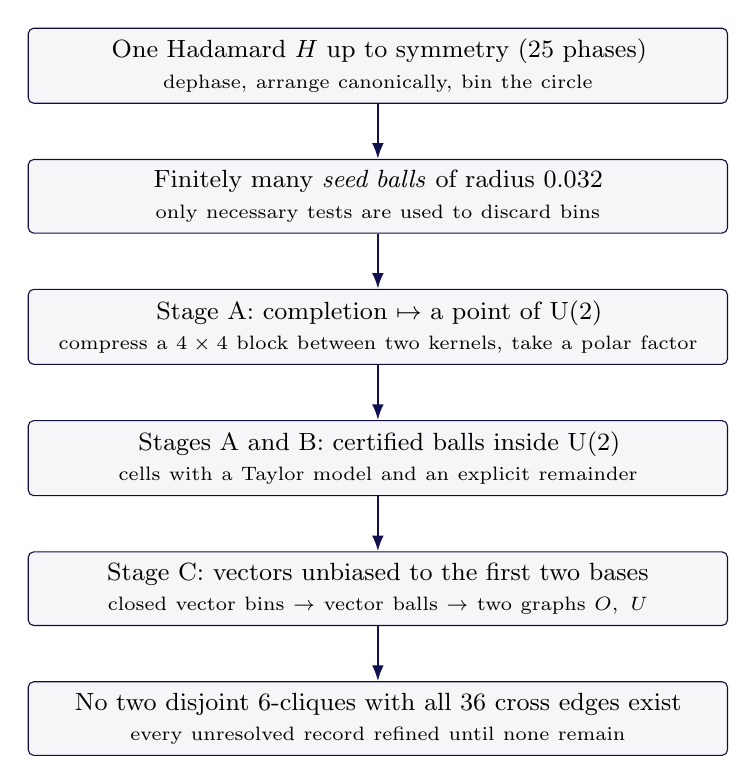
\begin{tikzpicture}[node distance=7mm,font=\small,
box/.style={draw=MidnightBlue!60!black,fill=MidnightBlue!4,rounded corners=2pt,
text width=8.6cm,align=center,inner sep=4pt,minimum height=9mm},
ar/.style={-{Latex[length=2mm]},thick,MidnightBlue!70!black}]
\node[box] (a) {One Hadamard $H$ up to symmetry (25 phases)\\
 \scriptsize dephase, arrange canonically, bin the circle};
\node[box,below=of a] (b) {Finitely many \emph{seed balls} of radius $0.032$\\
 \scriptsize only necessary tests are used to discard bins};
\node[box,below=of b] (c) {Stage A: completion $\mapsto$ a point of $\U(2)$\\
 \scriptsize compress a $4\times4$ block between two kernels, take a polar factor};
\node[box,below=of c] (d) {Stages A and B: certified balls inside $\U(2)$\\
 \scriptsize cells with a Taylor model and an explicit remainder};
\node[box,below=of d] (e) {Stage C: vectors unbiased to the first two bases\\
 \scriptsize closed vector bins $\to$ vector balls $\to$ two graphs $O,\ U$};
\node[box,below=of e] (f) {No two disjoint $6$-cliques with all $36$ cross edges exist\\
 \scriptsize every unresolved record refined until none remain};
\foreach \x/\y in {a/b,b/c,c/d,d/e,e/f} \draw[ar] (\x) -- (\y);
\end{tikzpicture}
\caption{The five stages. Each arrow is a cover step: the next stage retains every exact candidate
the previous stage could have produced, possibly with room to spare. Exclusions happen inside each
stage, never between them.}
\label{fig:pipeline}
\end{figure}

\begin{paperbox}
Section 1.2 and Figure 1 of the preprint state this sequence in the same terms. Section 7 turns it
into a statement about one execution, and Appendix A supplies the arithmetic contract that makes
each label of the tree true.
\end{paperbox}

\section{The five steps in more detail}

\noindent\emph{A note on numbering.} Citations of the form \S2.3, Lemma~2.7, Proposition~2.10,
Lemma~3.4, Theorem~7.1 are the \emph{preprint's} own numbers, not this document's. The two schemes
collide often enough to be a nuisance --- this document's Lemma~3.2 is the preprint's Lemma~2.2, while
the preprint's Lemma~3.2 is cited below as exactly that --- so the citation says ``the preprint's''
wherever a collision is possible.

\subsection*{Step 1. From a continuum to finitely many balls (Section 2)}

After dephasing, look only at the first two rows and columns of $H$; this is the preprint's
equation (3.1):
\[
H'=\begin{pmatrix}E'&B'\\ C'&D'\end{pmatrix},\qquad
E'=\begin{pmatrix}1&1\\1&a\end{pmatrix},\quad
B'=\begin{pmatrix}1&1&1&1\\ b_0&b_1&b_2&b_3\end{pmatrix},\quad
C'=\begin{pmatrix}1&c_0\\ \vdots&\vdots\\ 1&c_3\end{pmatrix},
\]
with $D'$ a full $4\times4$ block. The nine numbers $(a,b_0,\dots,b_3,c_0,\dots,c_3)\in\mathbb T^9$
are called the \emph{seed}. Nothing is known about $D'$ yet.

Two observations reduce $\mathbb T^9$ to finitely many boxes.

\emph{A canonical order.} Call the \emph{gap} of a finite set of points on the circle the length of
the largest arc containing none of them, and count repeated points with multiplicity. Among all pairs
of rows and all pairs of columns of $H'$, take a pair whose six phase differences have the smallest
gap; transpose if the pair is a column pair, and permute rows so that it is the first two rows. Then
order the six phases of that pair around the circle, starting immediately after one of its largest
gaps, and write them as $0,e(x_1),\dots,e(x_5)$ with $e(t)=\exp(2\pi i t)$. If the orientation
condition $x_1\le x_5-x_4$ fails, interchange the two rows and reverse the ordering, which replaces
$x_i$ by $x_5-x_{5-i}$ and makes it hold. The outcome is
\[
0\le x_1\le\dots\le x_5\le 1,\qquad g_x=1-x_5,\qquad x_1\le x_5-x_4 ,
\]
so the largest gap of the list sits on the arc between $x_5$ and $0$, and it has length $g_x$. Now
choose one of the five noninitial columns, move it to second position and permute the last four rows;
the second column then has phases
\[
y=(0,\xi,y_2,y_3,y_4,y_5),\qquad 0\le y_2\le y_3\le y_4\le y_5\le1,
\]
where $\xi$ is the selected entry of $x$ --- the phase shared by the two lists --- and $g_y\ge g_x$.
Orthogonality of the first two rows is the vanishing sum $\sum_{j}e(x_j)=0$, orthogonality of the
first two columns is $\sum_j e(y_j)=0$, and these two identities are the only analytic information
carried to the next stage. That such an arrangement exists for every exact Hadamard matrix is
Lemma~2.4 of the preprint.

\emph{Bins.} Cut $[0,1]$ into $N=112$ closed bins of width $w=1/N$. A sorted list then has
nondecreasing bin indices, so each exact $H$ determines a finite tuple
\[
(a,b,c,d,\ell)\ \text{for the first list},\qquad (s,b_1',b_2',b_3',b_4')\ \text{for the second},
\]
with the shared entry remembered as an interval rather than a number. There are finitely many such
tuples; each is a box in $\mathbb T^9$, and each box contains its rational midpoint, the \emph{seed
centre}. A box is kept only if it survives three necessary tests, each with an explicit margin so
that the test is valid for the whole box and not only its midpoint:
a \emph{gap} comparison (Lemma~2.6), a \emph{vanishing-sum} test, which says that the five phases in
a row satisfy $1+\sum_j e(u_j+\Delta_j)=0$ and hence the deviation of the midpoint sum from $-1$ is
bounded by $\tfrac{5\pi}{4}w^2$ (Lemma~2.7), and an intersection of \emph{shared-displacement}
intervals for the phase common to the two lists (Lemma~2.8).

Their common mechanism is the preprint's Lemma~2.5, and it is worth isolating: if every point of one
circular multiset is matched to a point of another at circular distance at most $\delta$, then the
gaps of the two multisets differ by at most $2\delta$. A filter proved for the \emph{centre} of a box
therefore constrains \emph{every} exact list in that box, which is exactly the transfer the invariant
of \S\ref{sec:shape} needs.

Finally a \emph{reuse} test throws away a box whose feasible part already sits in a radius-$0.032$
ball about a centre retained earlier (Lemma~2.9). The output is the preprint's Proposition~2.10:

\begin{claim}
the retained centres, each with a recorded chosen position, cover the seed coordinates of every exact
complex Hadamard matrix, up to the equivalences of Lemma~\ref{lem:equiv}, by closed Euclidean balls of
radius $0.032$.
\end{claim}

The constant is not magic: a box has side $w$ in nine coordinates, so its circumradius is
$\tfrac{\sqrt 9}{2N}=\tfrac{3}{224}<0.032$, and a box that is not absorbed by an earlier centre
contributes its own midpoint as a new centre. That is the entire content of the covering statement;
everything before it is there to make the list of boxes short enough to visit.

\begin{ideabox}
The phase circle is a compact group, so the only way to make it finite is to quotient and to cut.
Quotienting uses the symmetries (permuting, rephasing, transposing, conjugating) plus a canonical
ordering that every exact matrix secretly satisfies. Cutting uses bins, and the bins are legitimate
because a box has a computable circumradius that a ball can swallow exactly.
\end{ideabox}

\subsection*{Step 2. The dimension collapse: every completion is a point of $\U(2)$ (Section 3)}

Fix a seed ball and, inside it, a seed centre; write the matrix in $2+4$ block form as above. The
seed controls $E'$, $B'$ and $C'$ up to their own small displacements, so the only real freedom left
sits in the $4\times4$ block $D'$, which carries sixteen phases. Counting equations against unknowns
suggests that completions are rare, but a count is not a description, and no count survives being
taken along a stratum where the orthogonality equations become dependent. The proof needs the solution
set \emph{identified}, and that is what makes the rest of the argument possible.

The identification uses two subspaces. The $2\times4$ block $B'$ has rank two, so its kernel
$\ker B'\subset\C^4$ is two-dimensional; likewise $\ker C'^*\subset\C^4$ is two-dimensional. Choose
orthonormal bases $K_B,K_C\colon\C^2\to\C^4$ of these two subspaces, and compress the unknown block
between them:
\[
Y=K_C^*\,D'\,K_B\ \in\ M_2(\C).
\]
The orthogonality equations of the $4\times4$ part, compressed the same way, give $6I-Y^*Y\ge0$ with
an explicitly bounded trace defect (the preprint's Lemma~3.2):
\[
6I-Y^*Y=K_B^*B'^*B'K_B+K_B^*D'^*P_C D'K_B\ \succeq\ 0,
\qquad
\tr(6I-Y^*Y)\le q .
\]
So all singular values of $Y$ are at most $\sqrt6$, and the total deficit from $\sqrt6$ is at most
$q$. If $q<6$, then $Y$ is invertible and its \emph{polar factor}
$V=Y(Y^*Y)^{-1/2}\in\U(2)$ satisfies
\[
\norm{Y-\sqrt6\,V}_{F}\le p:=\frac{q}{\sqrt6+\sqrt{6-q}} .
\]
In the parameter range actually used, $q<0.32$, so $p\lesssim 0.09$: the compressed block is a fixed
distance from a rigid rotation, not merely close to one.

\begin{ideabox}
This is the single most important structural step, and it is worth restating without symbols. Of the
25 phases of a dephased Hadamard matrix, nine are the seed and sixteen are the block $D'$. The
orthogonality equations see $D'$ only through the way it acts between two fixed two-dimensional
subspaces, so they see only a $2\times2$ matrix, and a $2\times2$ matrix satisfying ``$Y^*Y$ is
almost $6I$'' is nothing but a rotation and a small amount of stretching. The set of rotations in two
complex dimensions is the compact group $\U(2)$, which has four real parameters. So a problem with
25 continuous unknowns becomes: \emph{nine numbers in a box, plus a point of a four-dimensional
compact group}. Every exact completion hands us such a point, so covering the group covers every
completion; and the group is small enough to be covered by finitely many cells.
\end{ideabox}

One subtlety deserves emphasis, because it is the reason Step 2 is written the way it is. The seed
centre need not be a genuine Hadamard matrix; the frames $K_B,K_C$ are computed from the centre and
then held \emph{fixed} throughout the ball. That is legitimate only because the estimates are uniform:
a frame check (singular values of $B_0$ bounded below, the preprint's Lemmas 3.1 and 3.5) either passes, in which
case every exact matrix in the ball is within $R_s$ of the centre and the frames are valid
throughout, or it fails, and the seed is retained as unresolved rather than excluded. A failed frame
check is never a proof of anything.

\subsection*{Step 3. Certified cells: a Taylor model with a true remainder (Sections 3--5)}

Next, cover $\U(2)$. Every $V\in\U(2)$ can be written, for a suitable phase $\alpha$ with
$0\le\alpha\le\tfrac12$, as
\[
V=e(\alpha)\begin{pmatrix} e(\beta)\cos(2\pi t) & e(\gamma)\sin(2\pi t)\\
-e(-\gamma)\sin(2\pi t) & e(-\beta)\cos(2\pi t)\end{pmatrix},
\qquad 0\le t\le\tfrac14,\quad 0\le\beta,\gamma\le1,
\]
because $e(-\alpha)V\in\SU(2)$, every element of $\SU(2)$ is $\begin{psmallmatrix}z&w\\-\bar w&\bar z\end{psmallmatrix}$
with $\abs z^2+\abs w^2=1$, and $\abs z,\abs w$ can be written as a cosine and a sine with
$t\in[0,\tfrac14]$. The range is thus a product of four intervals, cut into a fixed grid of closed
cells, and each cell has a midpoint $U$ and a displacement
$\theta=(\theta_\alpha,\theta_t,\theta_\beta,\theta_\gamma)$ with $\abs{\theta_j}\le h=\pi/N_u$.

The estimates that make the grid usable are uniform Taylor bounds (the preprint's Lemma~3.4):
\begin{equation}\label{eq:taylor}
\norm{V-U}_{\Frob}\le\sqrt6\,h,\qquad
\norm{V-U-\dd U[\theta]}_{\Frob}\le\frac{\sqrt{42}}{2}h^2 .
\end{equation}
The second one is the useful one. It says that inside a cell, the exact rotations are within
$O(h^2)$ of a \emph{linear} model, uniformly, with a constant that is computed by differentiating the
four entries of the parametrisation. So a test designed for exact points can be run on the linear
model and then made true for the whole cell by inflating the tolerance; and the inflation is
quadratic in the cell width, which is small.

Stage B (Section 5) refines this. Instead of a box in the four angular coordinates, each retained
ball carries numerical approximations to the \emph{tangent} directions of the equations that a
completion must satisfy; a verified residual identity bounds the normal component of every exact
displacement by its tangential coordinates. Covering the tangential coordinates and adding the normal
bound gives smaller balls covering exactly the same exact solutions. No parametrisation of the
solution manifold is needed, and none is available: the point is that a curved piece of surface can
be covered by flat patches of known thickness.

\begin{ideabox}
Two operations, no geometry. \emph{Linearise}, so that the region's worth of points is described by
one model; \emph{inflate}, so that the model's failure to be exact is absorbed into the radius of a
ball that provably still contains everything. A computer proposes the model, the inequality certifies
it, and the certificate is the inequality --- not the computer's arithmetic. This is why the preprint
insists that a floating-point centre need not be a Hadamard matrix and a numerical linear solve need
not be accurate.
\end{ideabox}

\subsection*{Step 4. The combinatorial core: two graphs and two cliques (Section 6)}

At this point, for every seed ball and every retained cell inside it, we have a closed ball $B$ in
$\U(2)$-space known to contain every completion that the seed can produce. Inside such a ball, the
question becomes concrete: which vectors $w\in\C^6$ are unbiased to both of the first two bases,
that is, satisfy $\abs{\inner{e_i}{w}}^2=\abs{\inner{h_j}{w}}^2=\tfrac16$ for all $i,j$ (with $h_j$
the columns of $H/\sqrt6$)? A third basis is six such vectors, orthonormal; a fourth basis is six
more, orthonormal among themselves, unbiased to the first two bases, and unbiased to the third ---
$36$ further conditions.

The proof covers the set of candidate vectors by \emph{vector balls}: first by binning the $36$
entrywise phases again, then by replacing each bin by a small Euclidean ball around a computed
candidate. These balls are the vertices of two graphs:
\[
\begin{aligned}
O&:\ \text{there is a possible orthogonal pair }(u,v),\\
U&:\ \text{there is a possible unbiased pair }(u,v).
\end{aligned}
\]
Both graphs are \emph{necessary-condition graphs}: an edge is retained whenever the hypothesis has not
been refuted, so $O$ and $U$ contain every genuine orthogonal, respectively unbiased, pair. Then
\begin{claim}
two further bases exist $\Longrightarrow$ $O$ contains two disjoint $6$-cliques (one for each of the
two bases) whose $36$ cross pairs are all edges of $U$.
\end{claim}
and the contrapositive of that implication is checked by finite enumeration. If the pattern is absent
from the (larger) graphs, it is absent from reality.

\begin{figure}[t]
\centering
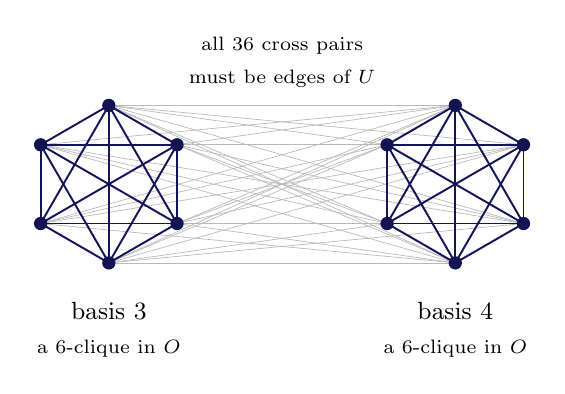
\begin{tikzpicture}[font=\small,dot/.style={circle,fill=MidnightBlue!75!black,inner sep=1.7pt}]
% the two hexagons: vertices of O-cliques
\foreach \k/\dx in {L/0,R/4.4}{
  \coordinate (\k1) at (\dx+0,1);
  \coordinate (\k2) at (\dx-0.866,0.5);
  \coordinate (\k3) at (\dx-0.866,-0.5);
  \coordinate (\k4) at (\dx+0,-1);
  \coordinate (\k5) at (\dx+0.866,-0.5);
  \coordinate (\k6) at (\dx+0.866,0.5);
}
% the 36 cross conditions
\foreach \i in {1,...,6}{\foreach \j in {1,...,6}{
  \draw[gray!55,line width=0.25pt] (L\i)--(R\j);}}
% the two cliques in O
\foreach \k in {L,R}{
  \foreach \i/\j in {1/2,1/3,1/4,1/5,1/6,2/3,2/4,2/5,2/6,3/4,3/5,3/6,4/5,4/6,5/6}{
    \draw[MidnightBlue!80!black,line width=0.7pt] (\k\i)--(\k\j);}
}
\foreach \k in {L,R}{\foreach \i in {1,...,6}{\node[dot] at (\k\i) {};}}
\node[align=center] at (0,-1.85) {basis 3\\[1pt]{\scriptsize a $6$-clique in $O$}};
\node[align=center] at (4.4,-1.85) {basis 4\\[1pt]{\scriptsize a $6$-clique in $O$}};
\node[align=center] at (2.2,1.55) {\scriptsize all $36$ cross pairs\\[1pt]\scriptsize must be edges of $U$};
\end{tikzpicture}
\caption{What two further bases would look like. Each basis is six pairwise orthogonal vectors of
$\C^6$, i.e.\ a hexagon of edges of $O$; every vector of the first must be unbiased to every vector of
the second, i.e.\ all $36$ cross pairs must be edges of $U$. The graphs are supersets of the true
relations, so a pattern that is absent from them is absent from reality.}
\label{fig:cliques}
\end{figure}

\begin{ideabox}
Locally the problem is easy and globally it is impossible, and the proof makes that dichotomy into
an object. Single vectors unbiased to two given bases are easy to come by --- for the
standard--Fourier pair they form a finite set that Grassl computed explicitly, and still no two
further bases exist --- but the twelve vectors needed for two more bases have to satisfy $15$ orthogonality conditions inside each basis and $36$ unbiasedness
conditions across them. The obstruction is therefore combinatorial rather than analytic, which is why
the last stage of the proof is a finite graph search and not another estimate.
\end{ideabox}

\subsection*{Step 5. One execution, no unresolved record (Section 7)}

Every seed, every refined ball and every initially unresolved record carries a record in a finite
control flow. A record ends in one of three states: excluded (a necessary condition failed with
margin), resolved (its completions were transferred to a certified ball and later excluded), or
unresolved. The theorem is the implication

\begin{claim}
a complete execution that terminates with no unresolved record certifies that no four mutually
unbiased bases exist in $\C^6$.
\end{claim}

That implication, not the run, is the mathematics of Section 7; the run is evidence that its
hypothesis holds. The preprint is explicit that the hypothesis is conditional on stated binary64
arithmetic and compiler behaviour, on one documented execution, and on the arithmetic contract of
Appendix A, where every test used anywhere above is shown to be evaluable with a stated margin. The
fallback loop is what makes the implication usable: an unresolved region is split and reprocessed,
and the execution is declared complete only when the list of unresolved records is empty.

\section{Why the estimates are ugly, and where}

Nothing above needed an estimate sharper than a circumradius or a Taylor remainder. The ugly parts
are all in service of the invariant --- each is an inequality whose only job is to make one node of
the decision tree true --- and a reader who wants to check the proof's logic can read the table below
in place of the paper.

\begin{center}
\small
\begin{tabular}{@{}p{3.5cm}p{5.4cm}p{5.4cm}@{}}
\toprule
\textbf{Paper} & \textbf{What it does} & \textbf{Why it is needed} \\
\midrule
\S2.1, Lem.~2.2 & rephasing, permutation, conjugation, transposition as symmetries & to fix eleven phases and to allow canonical ordering \\
\S2.2, Lem.~2.4 & canonical arrangement of the nine phases & every exact $H$ has a sorted, dephased representative \\
\S2.2, Lem.~2.5--2.6 & gap stability and midpoint gap filters & discard bins without losing exact points \\
\S2.3, Lem.~2.7--2.8 & vanishing-sum test and shared-displacement intervals & the two remaining necessary tests on a seed box \\
\S2.4, Lem.~2.9 & certified reuse of previous centres & keeps the number of retained balls small \\
\S2.4, Prop.~2.10 & the covering statement & Step 1 is complete: every $H$ is in some ball of radius $0.032$ \\
\S3.1, Lem.~3.1--3.5 & frames from two kernels; singular-value bounds & the frames are fixed and legitimate throughout a ball \\
\S3.2, Lem.~3.2 & polar comparison, $q$ and $p$ & every completion gives a point of $\U(2)$, quantitatively \\
\S3.3, Lem.~3.3--3.4 & parametrise $\U(2)$; Taylor with remainder & a finite grid of cells, each certified uniformly \\
\S3.5--3.6 & linearisation remainder; necessary flatness & Stage B: balls shrink without losing solutions \\
\S4 & certified phase balls and their atlas & transport balls between seeds; merge into one atlas \\
\S5 & refinement relations, tangent grids, radius growth & the fallback: unresolved cells get smaller and die \\
\S6 & phase bins, vector balls, $(O,U)$ graphs, edge tests & the combinatorial exclusion of the last two bases \\
\S7 & records, control flow, finite-execution implication & the theorem as a statement about one completed run \\
App.~A & every constant, margin and rounding bound & the arithmetic contract that each node relies on \\
\bottomrule
\end{tabular}
\end{center}

Two comments on method. First, the proof is a \emph{certified} computation rather than a verified one
in the sense of a proof assistant: the computer proposes centres, kernels, tangent directions and
graph edges, and hand-proved inequalities accept or reject them. The distinction matters because it
tells you where to look if something is wrong: not in the linear algebra, which is elementary
throughout, but in the constants of Appendix A and in the control flow of Section 7 that claims every
region was visited. Second, the inconvenient truth is that the theorem is only as strong as its
arithmetic hypotheses; the preprint says so in the statement of Theorem 1.1, and any honest summary of
the result has to repeat it. A companion paper proves a weaker bound, $N(6)\le 5$, by exact
arithmetic, and parts of the surrounding framework have been formalised; as of writing, the upper
bound of three rests on the documented execution and has not been through peer review.

\section{Exercises}

\begin{exercise}\label{ex:doubly}
Prove that for orthonormal bases $\mathcal B,\mathcal C$ the matrix $P_{ij}=\abs{\inner{b_i}{c_j}}^2$ is
doubly stochastic. Deduce that ``unbiased'' is the strongest possible statement of the form ``$P$ is
uniform'', and that if $d=2$ and one entry of $P$ equals $\tfrac12$ then all four do.
\end{exercise}

\begin{exercise}\label{ex:rephase}
Show that multiplying the $i$-th row of a Hadamard matrix $H$ by a unit scalar $u_i$ and the $j$-th
column by $v_j$ leaves the family $\{\text{standard},\ \text{columns of }H/\sqrt6\}$ unbiased, and
corresponds to composing the two bases with diagonal unitaries. Conclude that eleven of the $36$
phases of $H$ are pure gauge.
\end{exercise}

\begin{exercise}\label{ex:d2had}
Show that every complex Hadamard matrix of order two is equivalent, under the operations of
Lemma~\ref{lem:equiv}, to $\begin{psmallmatrix}1&1\\1&-1\end{psmallmatrix}$; then show that $\C^2$
admits exactly three mutually unbiased bases. (Hint for the second part: after normalising two bases
to $I$ and $H/\sqrt2$, the phase of the second basis is the only freedom left, and the third basis
is forced up to finitely many choices.)
\end{exercise}

\begin{exercise}\label{ex:tensor}
Prove \eqref{eq:tensor}, and deduce that if $\mathcal A$ and $\mathcal B$ are unbiased pairs in
$\C^{d_1}$ and $\C^{d_2}$ then $\{a\otimes b\}$ and $\{a'\otimes b'\}$ are unbiased in
$\C^{d_1d_2}$. Conclude $N(d_1d_2)\ge\min\{N(d_1),N(d_2)\}$ and hence $N(6)\ge3$; explain why this
construction cannot give a fourth basis in $\C^6$.
\end{exercise}

\begin{exercise}\label{ex:polar}
Let $Y\in M_2(\C)$ satisfy $6I-Y^*Y\succeq0$ and $\tr(6I-Y^*Y)\le q<6$. Writing the singular values
as $\sigma_j=\sqrt{6-\ell_j}$ with $\ell_j\ge0$, show $\ell_1+\ell_2\le q$ and hence
\[
\norm{Y-\sqrt6\,V}_{\Frob}\le\frac{q}{\sqrt6+\sqrt{6-q}},\qquad V=Y(Y^*Y)^{-1/2}\in\U(2).
\]
This is the quantitative form of ``every completion is a point of $\U(2)$''.
\end{exercise}

\begin{exercise}\label{ex:logic}
Suppose $O$ and $U$ are graphs on a finite set of balls containing every genuine orthogonal and
unbiased pair respectively. Show that the absence of two disjoint $6$-cliques in $O$ with all $36$
cross edges in $U$ implies that no two further bases exist whose vectors lie in those balls. Then
explain why the converse direction is \emph{not} available: a pattern present in $O,U$ proves nothing.
(This asymmetry is the whole reason the proof is an exclusion argument and not a search for
solutions.)
\end{exercise}

\begin{exercise}\label{ex:count}
Count the real dimensions: a dephased $6\times6$ Hadamard matrix has $25$ free phases, its first two
rows and columns carry nine of them, and the remaining $4\times4$ block has sixteen. With a $2+4$ split
the blocks $B'$ and $C'^*$ have rank two, so their kernels in $\C^4$ are two-dimensional and the
compressed block is $2\times2$ --- whatever the dimension of the ambient space. Explain why the
reduction of Step~2 is useful only because $\U(2)$ is compact and has just four real parameters: a
compact group of low dimension can be covered by finitely many cells, and that is all the argument
needs.
\end{exercise}

\end{document}
